\documentclass{beamer-control}
\usepackage{beamer-control-singlefile}
\INCLUDEONLY{Introduction}
\begin{document}
\CONCEPT{Introduction}

\begin{SUMMARY}
\begin{itemize}
\item What is a Dynamical System?
\item What is Feedback and Feedforward?
\item What is Control?
\item Feedback Properties (or `why control?')
\item Simple Forms of Feedback
\item Broader Concepts of Control
\end{itemize}
\vfill References:
\begin{itemize}
\item \astrom{Chapter 1}
\item \url{https://engineeringmedia.com/map-of-control}
\end{itemize}
\end{SUMMARY}

\begin{frame}
\frametitle{What is a Dynamical System?}

Dynamical systems have variables (or \emph{states}) $\mathbf{x}$ which change over time:
\begin{align}
\dot \mathbf{x}(t) = f(\mathbf{x},t)
\end{align}
They generally do not exist alone, and include inputs $\mathbf{u}$:
\begin{align}
\dot \mathbf{x}(t) = f(\mathbf{x},t) + \mathbf{u}(t)
\end{align}
Dynamical systems can be linear or nonlinear, solvable analytically or only numerically.

\bigskip
\uncover<2>{\emph{\alert{We must understand dynamical systems before control systems.}}}
\end{frame}

\begin{frame}{What is Feedback? \AMref{§1.1}}
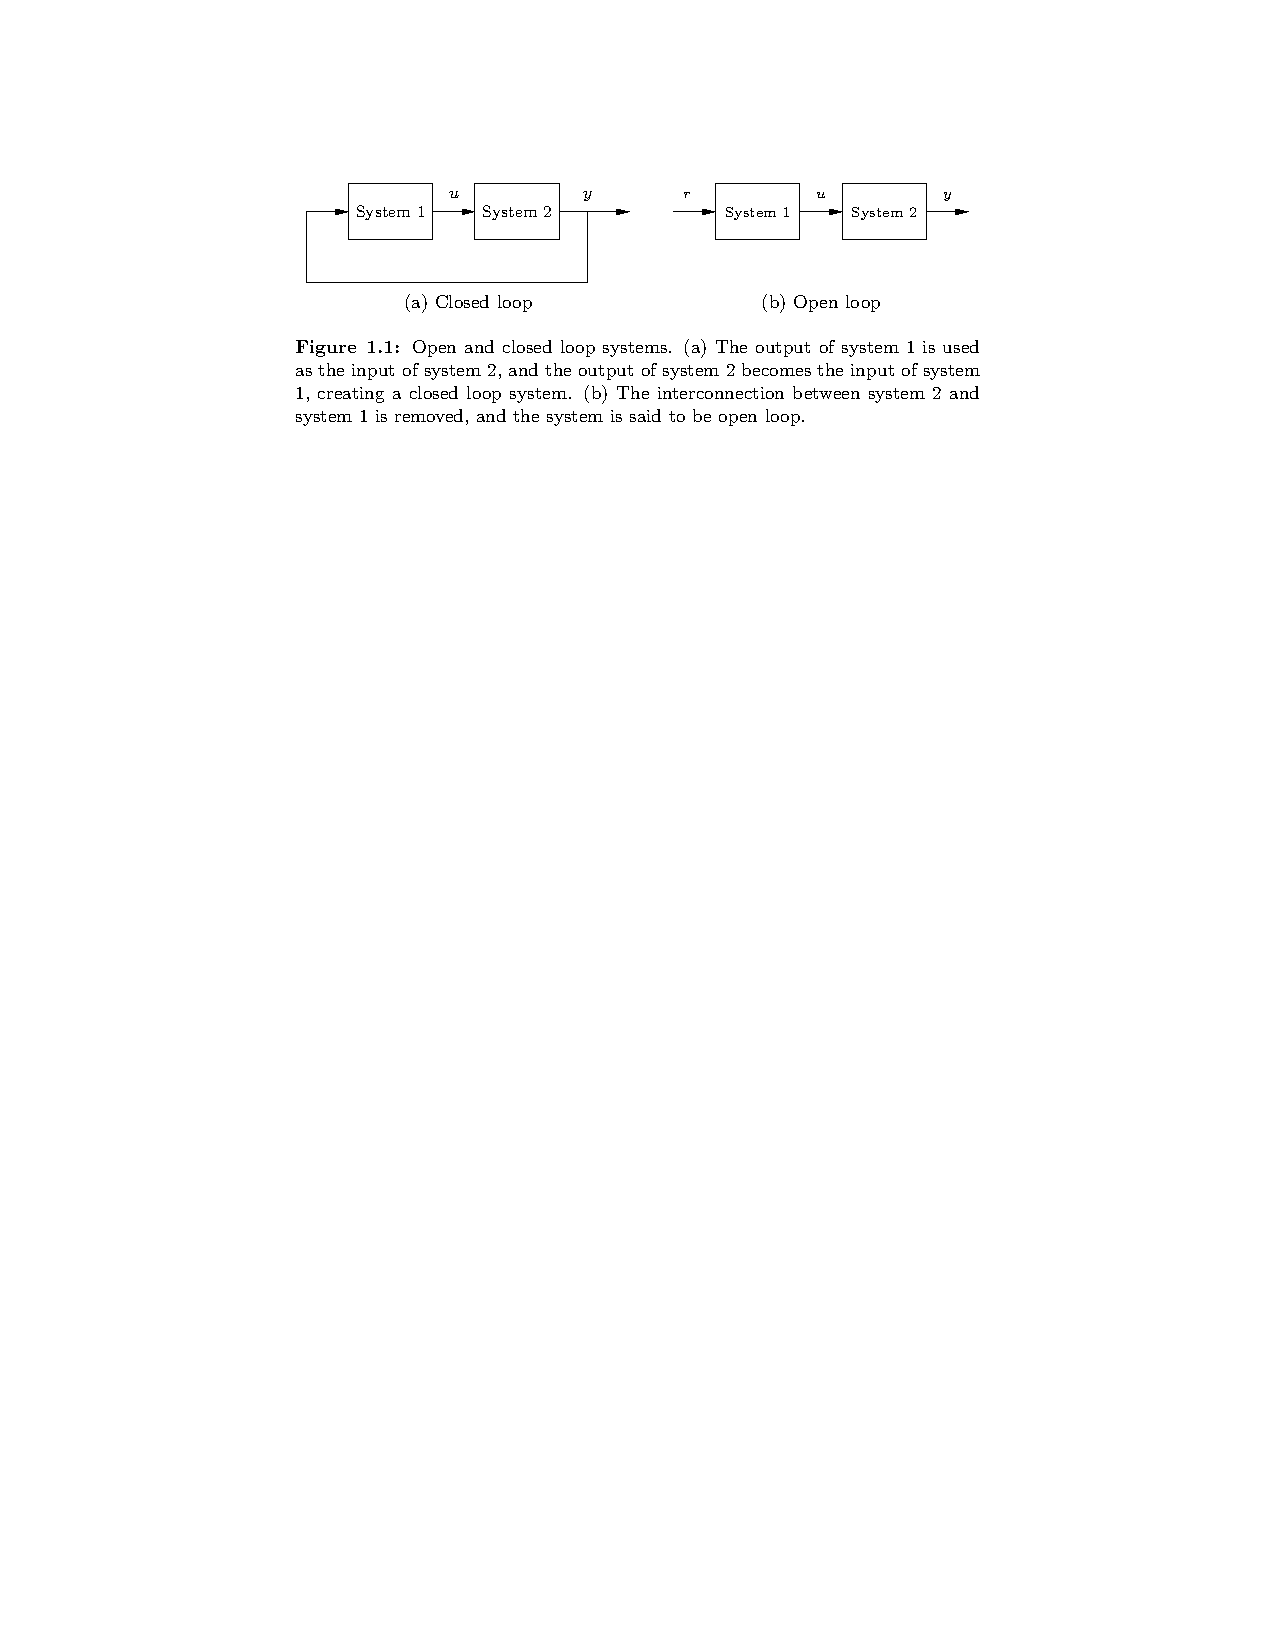
\includegraphics[width=\linewidth]{figure1.1}
\end{frame}

\begin{frame}{What is Feedforward? \AMref{§1.2}}
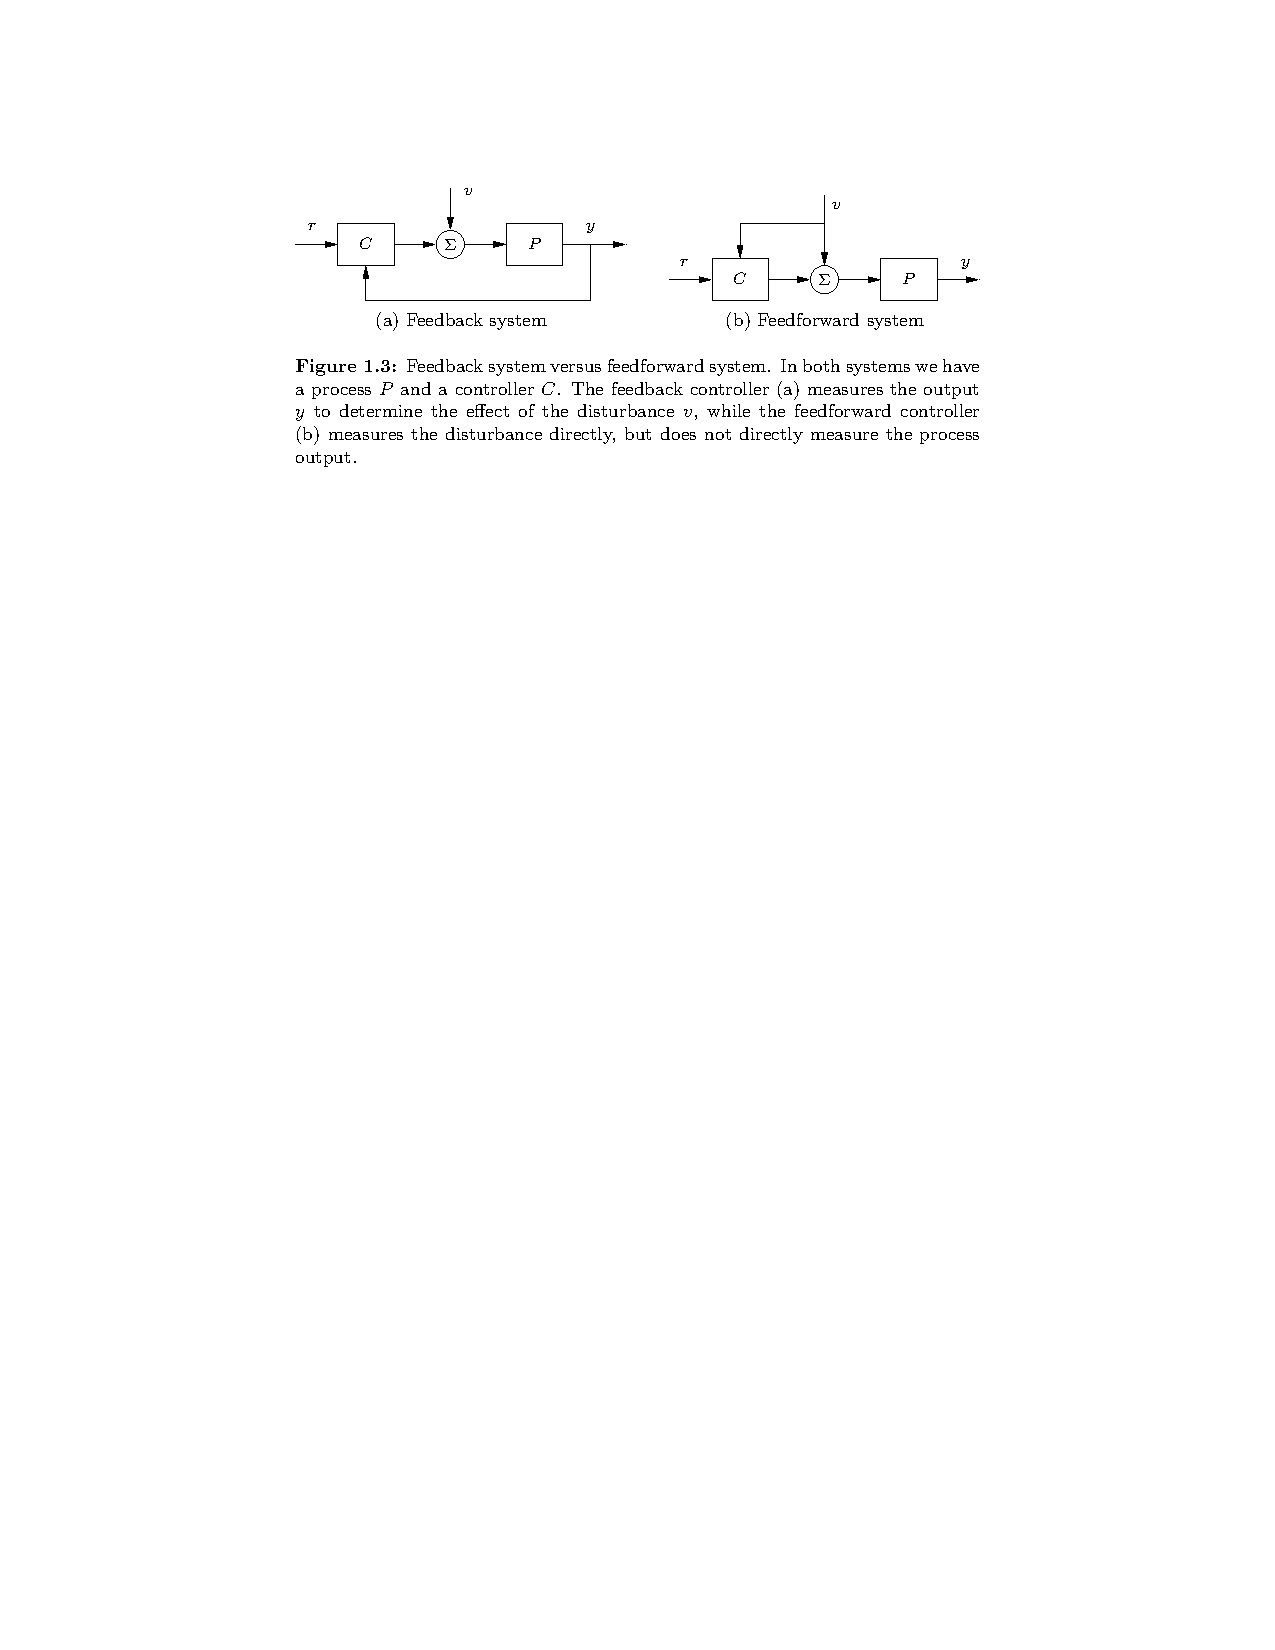
\includegraphics[width=\linewidth]{figure1.3}
\end{frame}

\begin{frame}{What is Control? \AMref{§1.3}}
Augmenting a system to change/improve its dynamics:
\begin{itemize}
\item Passive control: adding a passive element (usually trivial)
\item Active control: adding a feedback (or feedforward) loop
\item Generally involves three elements:
\begin{itemize}
\item Sensors (can't control what you don't know)
\item Controller (calculate what to do based on the state)
\item Actuators (effect the desired changed)
\end{itemize}
\end{itemize}
\end{frame}

\begin{frame}
\frametitle{The cruise control feedback system}

\end{frame}

\begin{frame}{Uses of Feedback and Control \AMref{§1.4}}
Control systems are truly multidisciplinary:
\begin{itemize}
\item Power systems (Elec Eng)
\item Process systems (Chem Eng)
\item Aerospace systems (Mech Eng)
\item Infrastructure systems (Civil/Environ Eng)
\item Economics (tariffs!)
\item Biology, Ecology, Climate Change \dots
\end{itemize}
\end{frame}

\begin{frame}
\frametitle{Feedback Properties \AMref{§1.5}}
\begin{itemize}
\item<only@1> General solution to asking an engineering system to respond to demands
\item<only@2> Robustness to uncertainty
\begin{itemize}
\item Rejection of disturbances
\item Mitigating sources of error
\item Adapting to changing conditions
\end{itemize}
\item<only@3> Design of dynamics
\begin{itemize}
\item Controlling stability (aerospace)
\item Precise control (robotics)
\end{itemize}
\item<only@4> Challenges
\begin{itemize}
\item Stability
\item Coupling
\item Complexity
\end{itemize}
\end{itemize}
\end{frame}


\begin{frame}
\frametitle{The canonical control block diagram}

\end{frame}


\begin{frame}
\frametitle{Simple Forms of Feedback \AMref{§1.6}}
\framesubtitle{On-Off Control}
\fbox{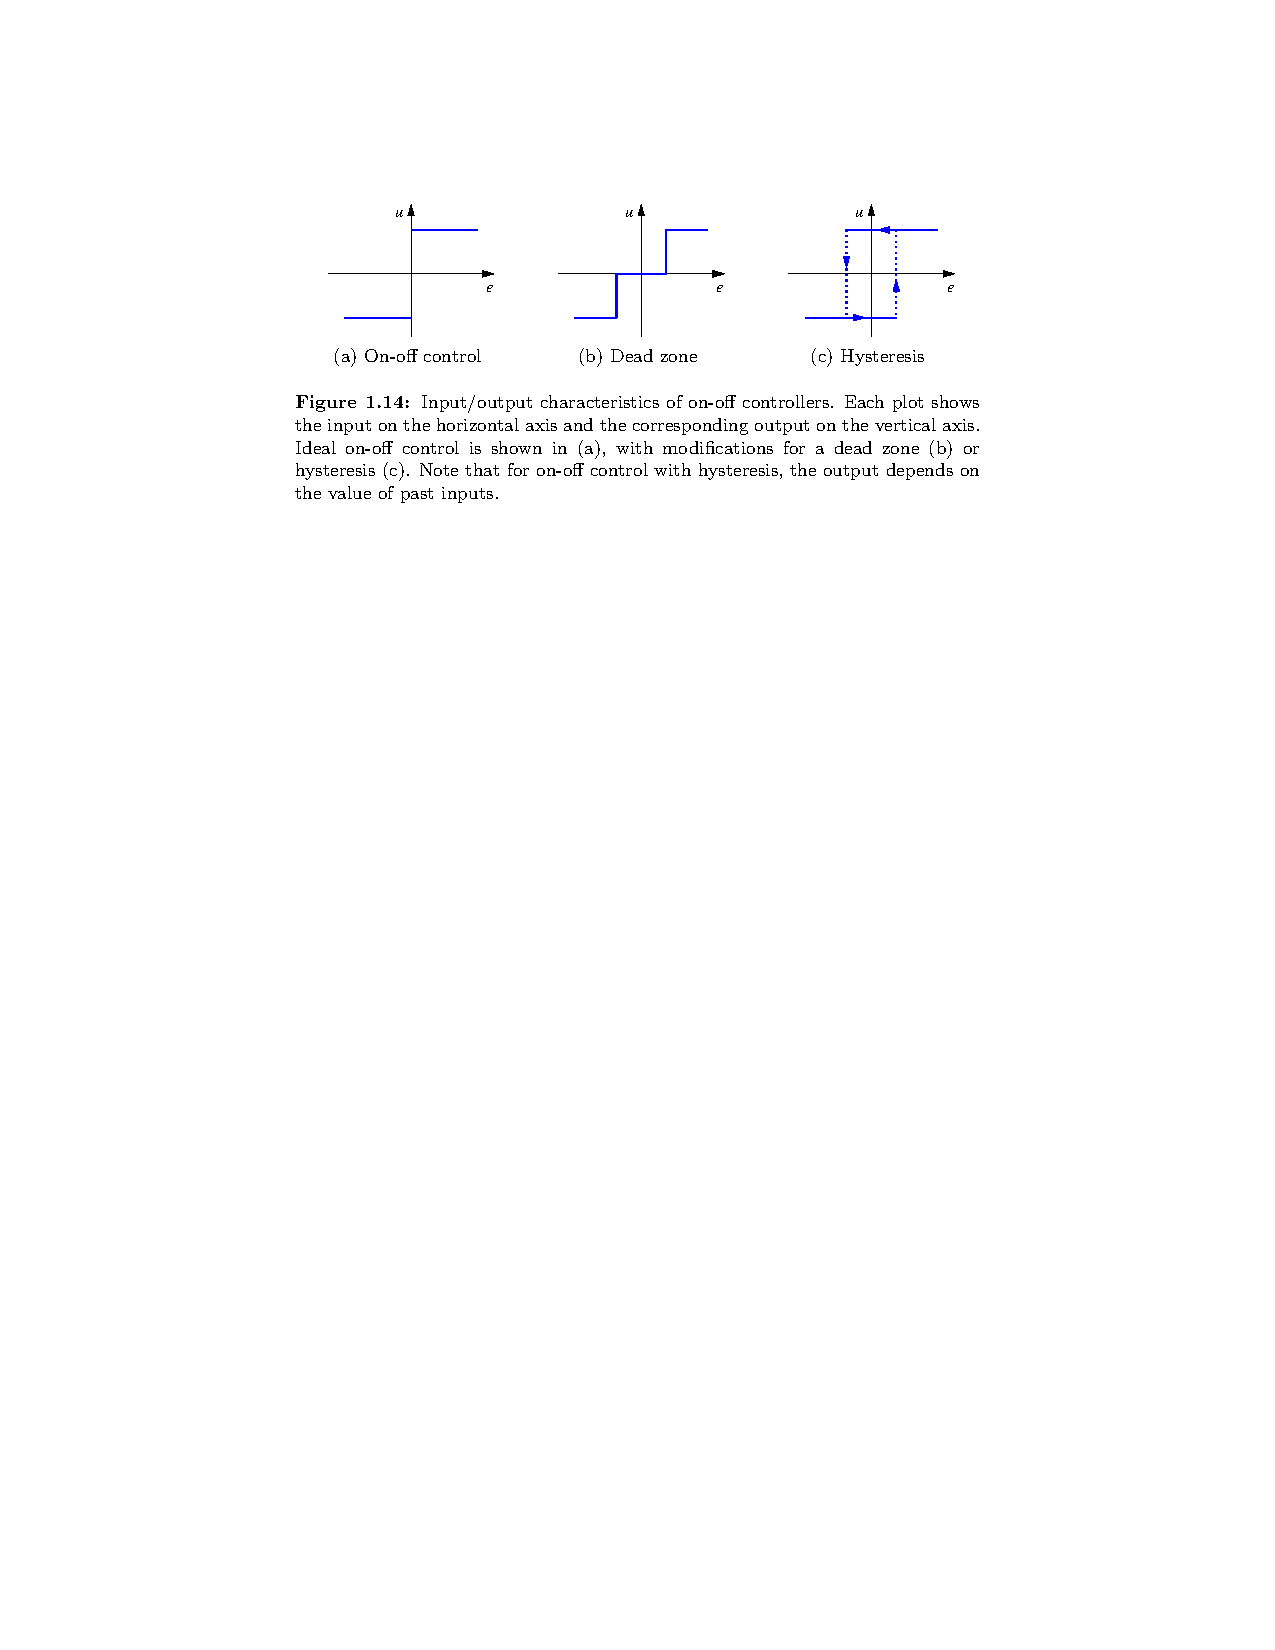
\includegraphics[width=\linewidth,trim=0 41 0 0,clip]{figure1.14}}
\begin{gather}
u(t) = \operatorfont{sign}(e)\, u_{\mathrm{max}}
\end{gather}
\end{frame}

\begin{frame}
\frametitle{Simple Forms of Feedback \AMref{§1.6}}
\framesubtitle{PID Control}
\fbox{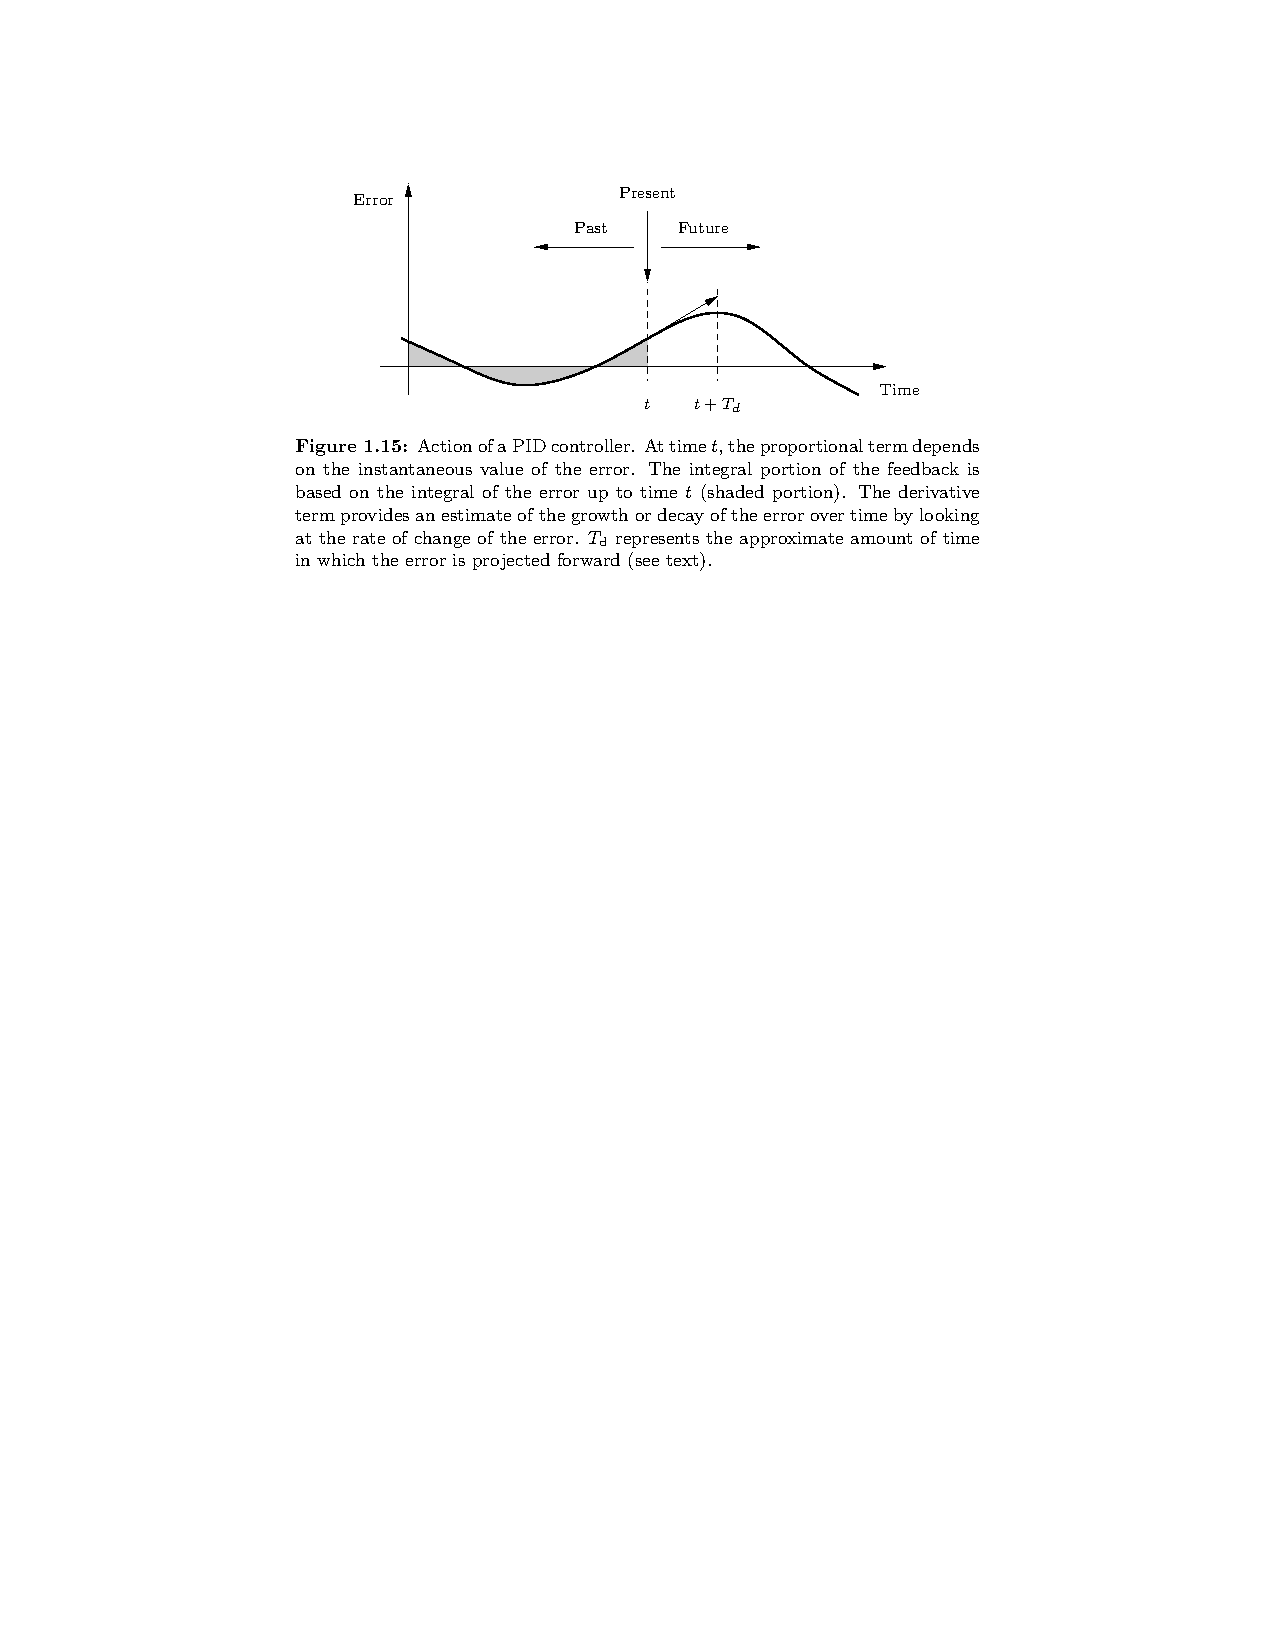
\includegraphics[width=\linewidth,trim=0 52 0 0,clip]{figure1.15}}
\vfil
\begin{gather}
u(t) = k_p e(t) + k_i \int_0^t e(\tau) \mathrm d\tau + k_d \frac{\mathrm d e(t)}{\mathrm d t}
\end{gather}
\end{frame}

\begin{frame}
\frametitle{Combining Feedback with Logic \AMref{§1.7}}
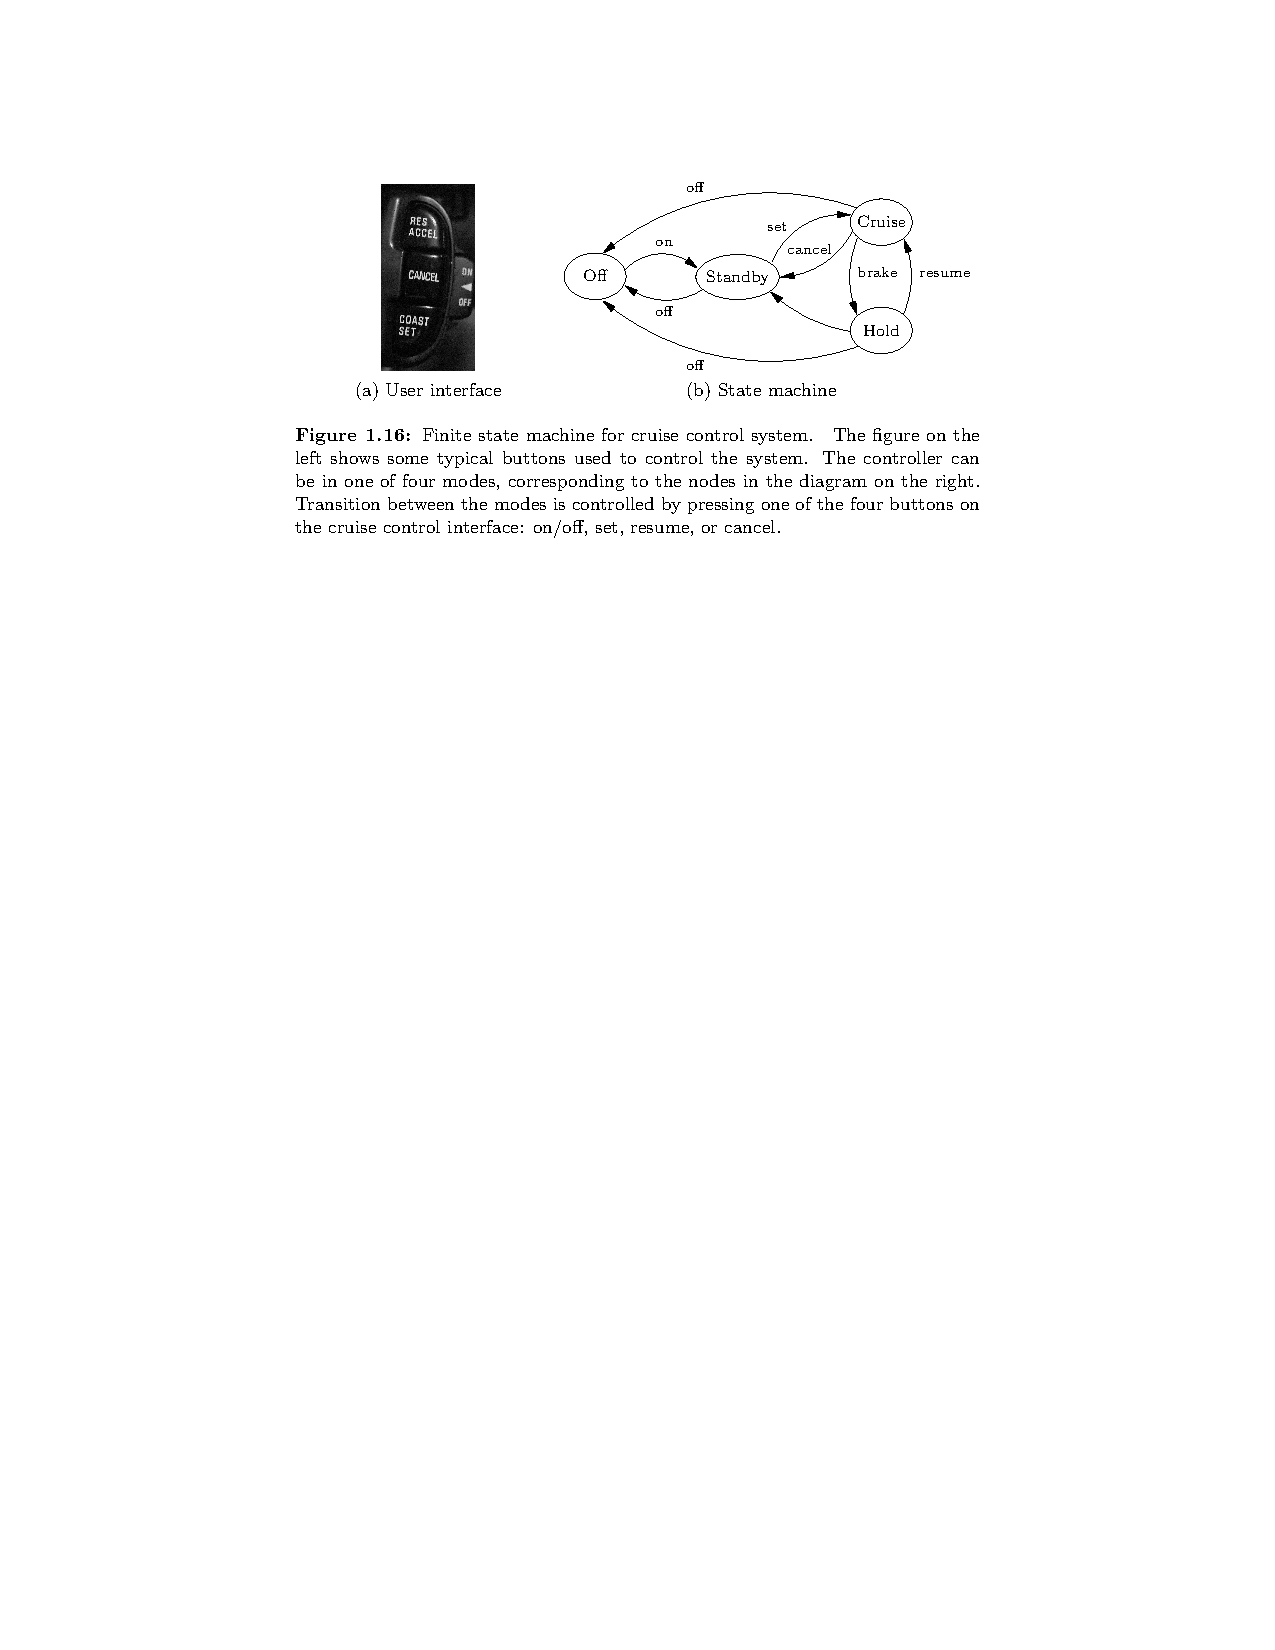
\includegraphics[width=\linewidth]{figure1.16}
\end{frame}

\begin{frame}
\frametitle{Control System Architectures \AMref{§1.8}}
\centering
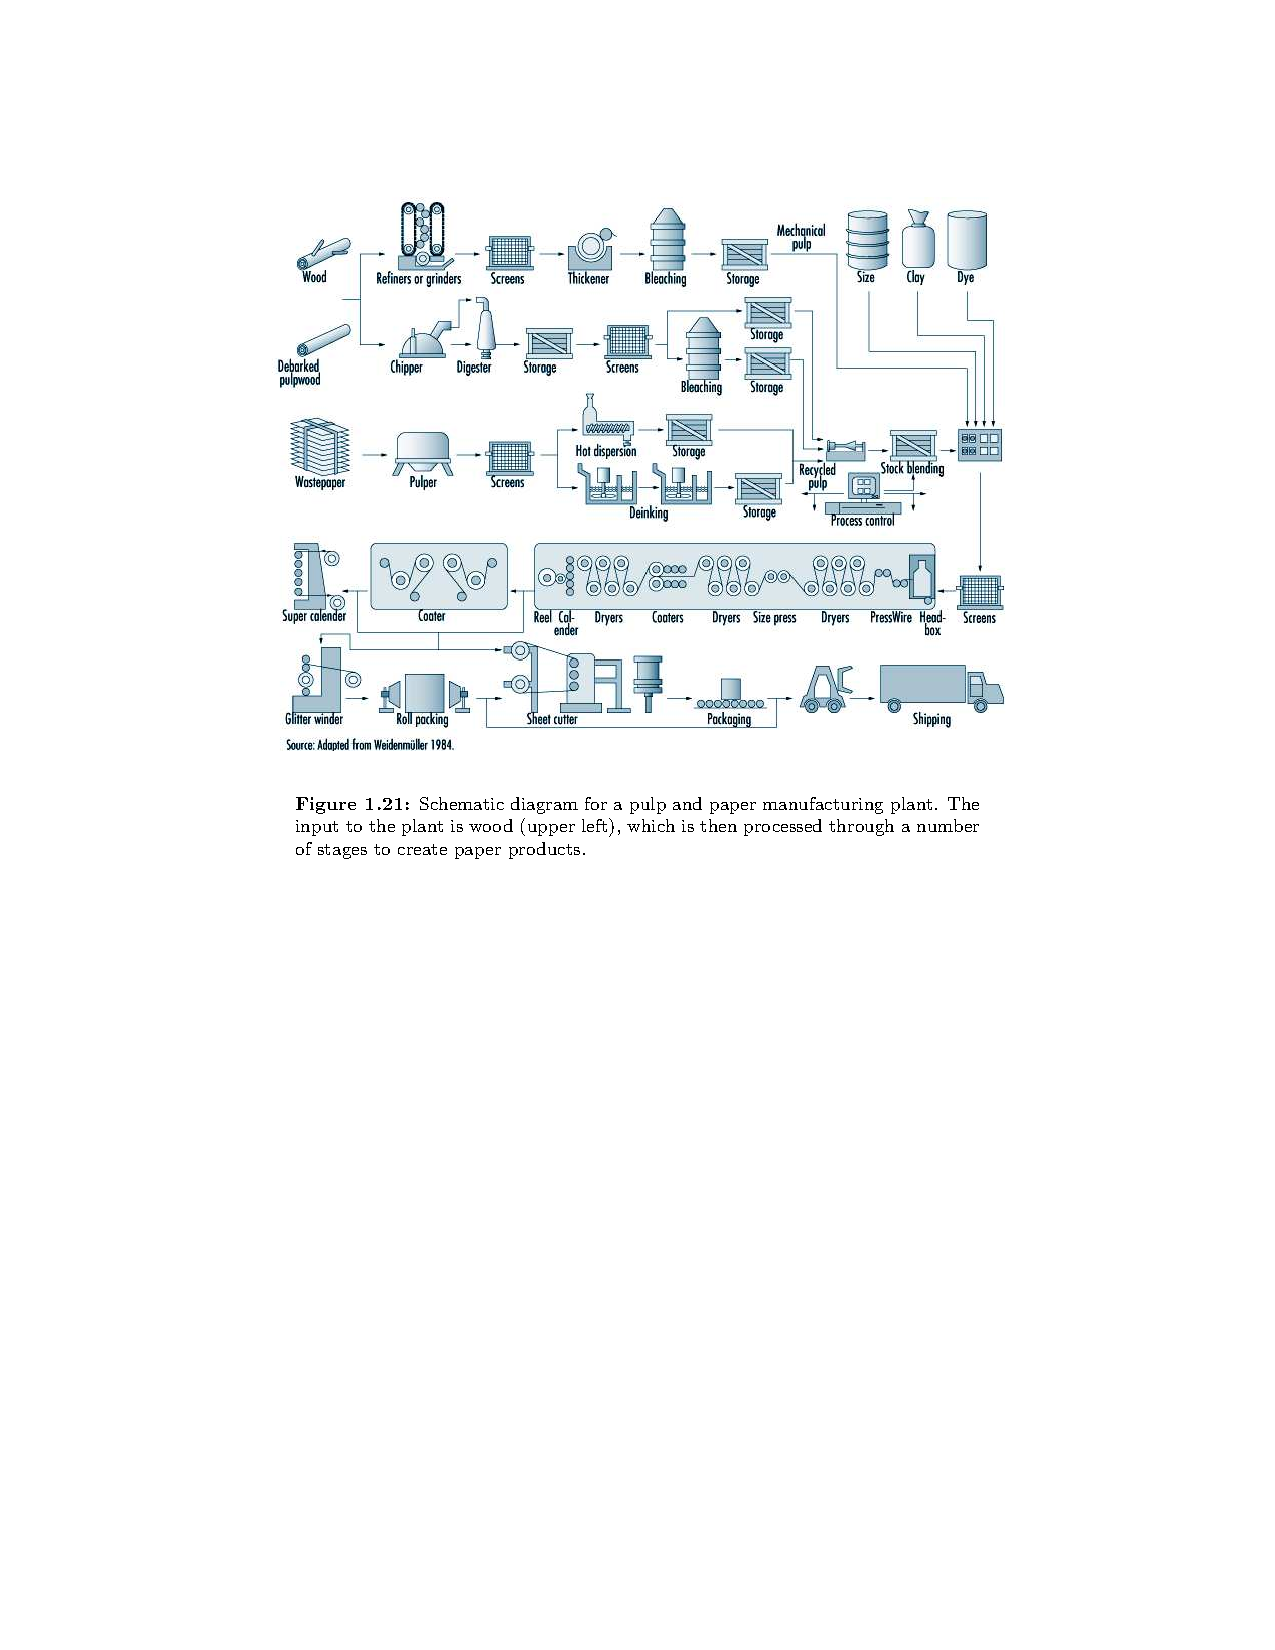
\includegraphics[width=0.8\linewidth]{figure1.21}
\end{frame}

\begin{frame}
\frametitle{Brian Douglas' Map of Control Theory}
\centering
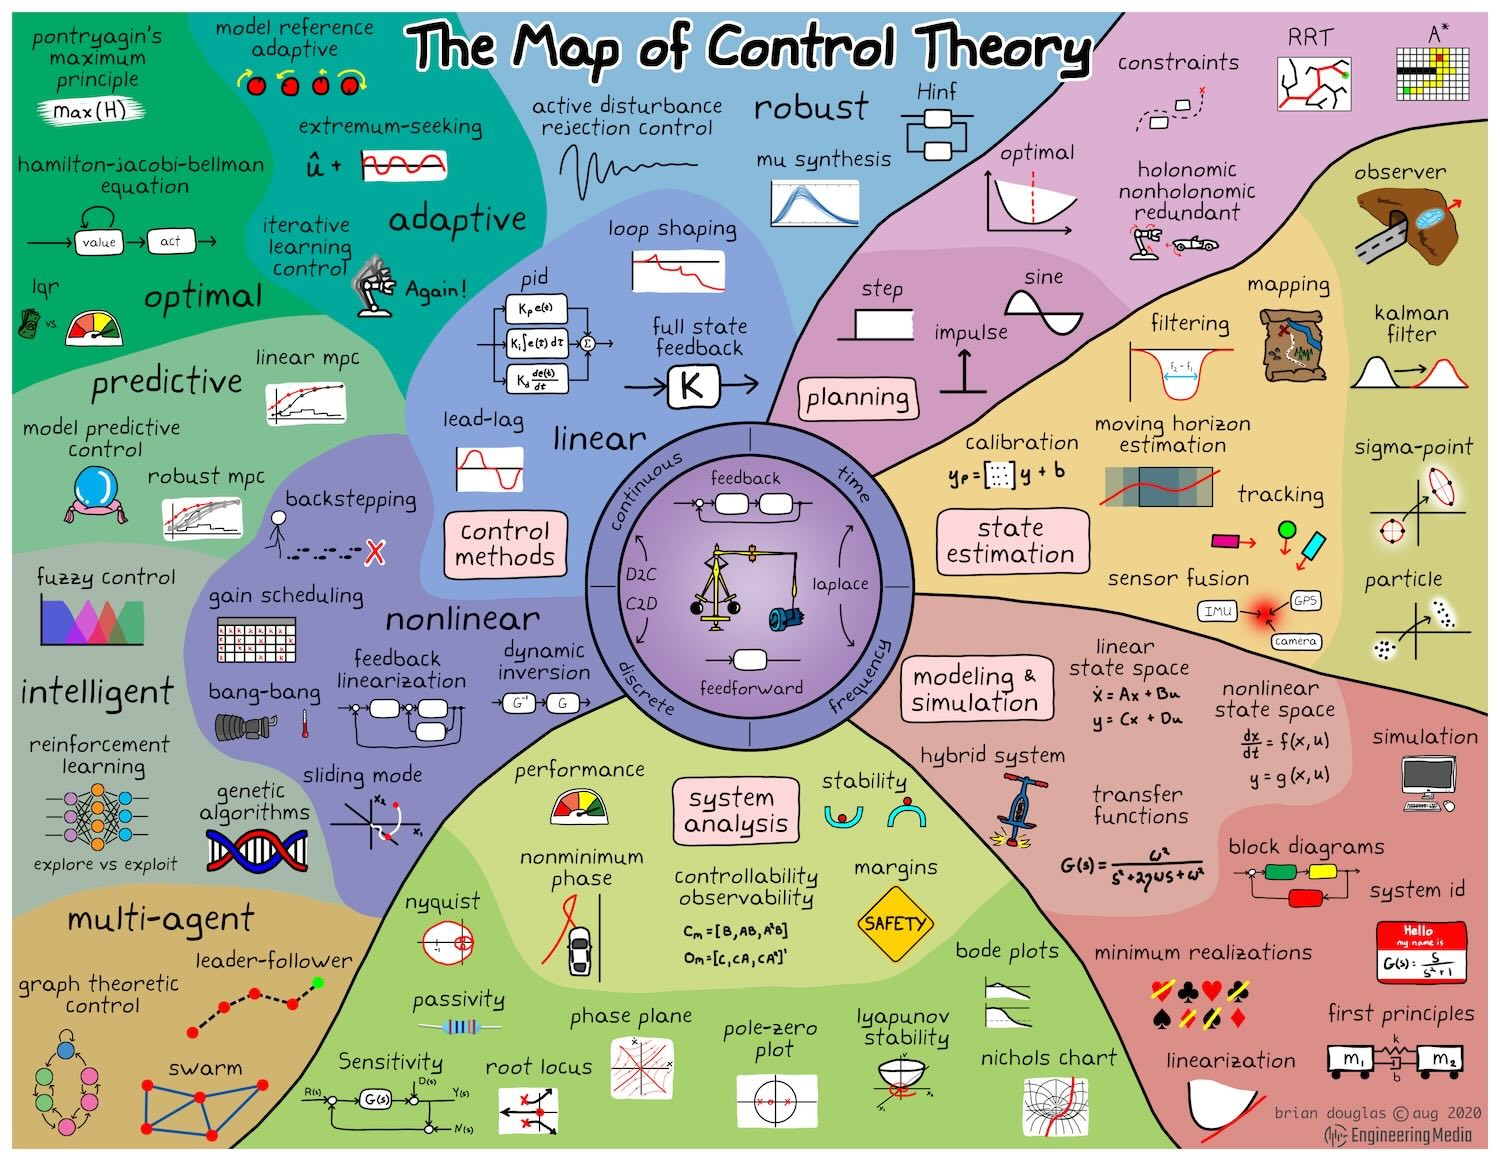
\includegraphics[width=0.90\linewidth]{Control_Map_ver5_wr}
\end{frame}

\SUMMARYFRAME
\FINALE

\end{document}
